\documentclass[12pt, fullpage,letterpaper]{article}

\usepackage[margin=1in]{geometry}
\usepackage{url}
\usepackage{amsmath}
\usepackage{graphicx}
\usepackage{tikz}
\usepackage{hyperref}

\newcommand{\semester}{Fall 2018}
\newcommand{\assignmentId}{1}
\newcommand{\releaseDate}{28 August, 2018}
\newcommand{\dueDate}{11 September, 2018}

\newcommand{\bx}{{\bf x}}
\newcommand{\bw}{{\bf w}}

\title{CS 5350/6350: Machine Learining \semester}
\author{Homework \assignmentId}
\date{Handed out: \releaseDate\\
  Due date: \dueDate}

\begin{document}
\maketitle

\section{Decision Trees}
\label{sec:q1}

\begin{enumerate}

\item~[6 points] In this warm-up question, you will be drawing decision trees for boolean functions. 
  \begin{enumerate}
  \item $(x_1 \wedge x_2) \vee \neg x_3$
    \begin{center}
    \begin{tikzpicture}[grow = down, level/.style={sibling distance=60mm/#1}, node/.style = {draw, circle}]
      \node[node] {$x_3$} % x_1
      child { node[node] {1}
        edge from parent node [above] {0}}
      child { node[node] {$x_1$} % x_2
        child { node[node] {$x_2$}
        	child { node[node] {1}
            	edge from parent node [above] {1}}
            child { node[node] {0}
            	edge from parent node [above] {0}}
          edge from parent node [above] {1}}
        child { node[node] {0}
          edge from parent node [above] {0}}
        edge from parent node [above] {1}};
    \end{tikzpicture}
  \end{center}
  \item $x_1$ xor $(x_2 \wedge x_3)$
  \begin{center}
    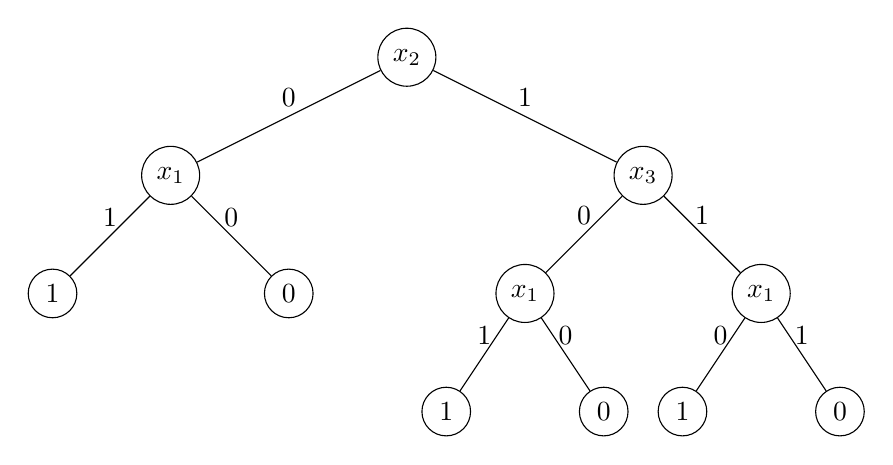
\begin{tikzpicture}[grow = down, level/.style={sibling distance=60mm/#1}, node/.style = {draw, circle}]
      \node[node] {$x_2$} 
      child { node[node] {$x_1$}
      	child { node[node] {1}
        	edge from parent node [above] {1}}
        child { node[node] {0}
        	edge from parent node [above] {0}}
        edge from parent node [above] {0}}
      child { node[node] {$x_3$}
        child { node[node] {$x_1$}
        	child { node[node] {1}
            	edge from parent node [above] {1}}
            child { node[node] {0}
            	edge from parent node [above] {0}}
          edge from parent node [above] {0}}
         child { node[node] {$x_1$}
        	child { node[node] {1}
            	edge from parent node [above] {0}}
            child { node[node] {0}
            	edge from parent node [above] {1}}
          edge from parent node [above] {1}}
        edge from parent node [above] {1}};
    \end{tikzpicture}
  \end{center}
  \item $x_1 \wedge (x_2 \vee (x_3 \wedge x_4))$
  \begin{center}
    \begin{tikzpicture}[grow = down, level/.style={sibling distance=60mm/#1}, node/.style = {draw, circle}]
      \node[node] {$x_1$} 
      child { node[node] {$x_2$}
      	child { node[node] {1}
        	edge from parent node [above] {1}}
        child { node[node] {$x_3$}
        	child { node[node] {$x_4$}
            	child { node[node] {1}
                	edge from parent node [above] {1}}
                child { node[node] {0}
                	edge from parent node[above] {0}}
            	edge from parent node [above] {1}}
            child { node[node] {0}
            	edge from parent node [above] {0}}
        	edge from parent node [above] {0}}
        edge from parent node [above] {1}}
      child { node[node] {0}
        edge from parent node [above] {0}};
    \end{tikzpicture}
  \end{center}
  \end{enumerate}

\item~[24 points] 
  Mark loves mangoes. Unfortunately he is lousy at picking ripe mangoes at the grocery. He needs your help.
  You need to build a decision tree that will help Mark decide if a mango is ripe or not. You need to make the decision based on
  four features described below:
  \begin{enumerate}
  \item\textbf{Variety} (\textit{Alphonso, Keitt or Haden}): Describes the variety of the mango.
  \item\textbf{Color} (\textit{Red, Yellow or Green}): Describes the color of the mango.
  \item\textbf{Smell} (\textit{Sweet or None}): Describes the smell of the mango.
  \item\textbf{Time} (\textit{One or Two}): Number of weeks since the mango was plucked.
  \end{enumerate}

  You are given the following dataset which contains data for 8 different mangoes. For each mango, the values of the above four features
  are listed. The label of whether the mango was ripe or not is also provided.

  \begin{table}[h]
    \centering
    \begin{tabular}{cccc|c}
      \hline
      Variety & Color    & Smell  & Time & Ripe?  \\ \hline
      Alphonso& Red      & None   & Two  & False  \\
      Keitt   & Red      & None   & One  & True   \\
      Alphonso& Yellow   & Sweet  & Two  & True   \\
      Keitt   & Green    & None   & Two  & False  \\
      Haden   & Green    & Sweet  & One  & True   \\
      Alphonso& Yellow   & None   & Two  & False  \\
      Keitt   & Yellow   & Sweet  & One  & False  \\
      Alphonso& Red      & Sweet  & Two  & True   \\ \hline
    \end{tabular}
    \caption{Training data for the mango prediction problem.}\label{tb-mango-train}
  \end{table}


  \begin{enumerate}
  \item~[5 points] How many possible functions are there to map these four features to a boolean decision? How many functions are consistent with the given training dataset?\\\\
  \textbf{Ans: }3 * 3 * 2 * 2 = 36 labels\\
	Total Functions: $2^{36}$\\
    We have 8 lines of known data hence there are 28 other combinations which may have differing labels. Hence $2^{28}$ functions are possible which are consistent with the given training set.
  \item~[3 points] What is the entropy of the labels in this data? When calculating entropy, the base of the logarithm should be base 2.\\
  \[Entropy = -\sum_{i} p_ilog\hspace{1mm}p_i\]

 \textbf{Ans: }Total Entropy (Ripe?):\\
 4/8 True, 4/8 False; Entropy = 1
  
  \item~[4 points] Compute the information gain of each feature and enter it into Table~\ref{tb-entropy-ig}. Specify upto 3 decimal places.
    \begin{table}[h]
      \centering
      \begin{tabular}{c|c}

        \hline
        Feature & Information Gain \\ \hline
        Variety & 0.156            \\
        Color   & 0.0615           \\
        Smell   & 0.1887           \\
        Time    & 0.0489           \\ \hline
      \end{tabular}
      \caption{Information gain for each feature.}\label{tb-entropy-ig}
    \end{table}\\
    \begin{itemize}
     \item Variety:\\
    Alphonso - 2/4 False, 2/4 True; Entropy = -1/2 log (1/2) - 1/2 log (1/2) = 1 \\
    Keitt - 1/3 False, 2/3 True; Entropy = -1/3 log (1/3) - 2/3 log(2/3) = -1/3 * (-1.585) - 2/3 * (-0.585) = 0.918 \\
    Haden - 1 - True 0 - False; Entropy = 0 \\
    Expected Entropy = 4/8 * 1 + 3/8 * 0.918 + 1/8 * 0 = 0.844\\
    \underline{Gain (Variety) = 1 - 0.844 = 0.156}\\
    \item Color:\\
    Red - 1/3 False, 2/3 True; Entropy = -1/3 log(1/3) - 2/3 log(2/3) = 0.918 \\
    Yellow - 2/3 False, 1/3 True; Entropy = 0.918\\
    Green - 1/2 False, 1/2 True; Entropy = 1\\
    Expected Entropy = 3/8 * 0.918 + 3/8 * 0.918 + 2/8 * 1 = 0.9385\\
    \underline{Gain (Color) = 1 - 0.9385 = 0.0615}\\
    \item Smell:\\
    None - 3/4 False, 1/4 True; Entropy = -3/4 log(3/4) - 1/4 log(1/4) = -3/4 (-0.415) - 1/4 (-2) = 0.8113\\
    Sweet - 1/4 False, 3/4 True; Entropy = -1/4 log(1/4) - 3/4 log(3/4) = 0.8113\\
    Expected Entropy = 4/8 * 0.8113 + 4/8 * 0.8113 = 0.8113\\
    \underline{Gain (Smell) = 1 - 0.8113 = 0.1887}\\
    \item Time: \\
    Two - 3/5 False, 2/5 True; Entropy = -3/5 log(3/5) - 2/5log(2/5) = -3/5 * (-0.737) - 2/5 * (-1.322) = 0.971
    One - 1/3 False, 2/3 True; Entropy = -1/3 log(1/3) - 2/3 log(2/3) = 0.918\\
  Expected Entropy = 5/8 * 0.971 + 3/8 * 0.918 = 0.9511\\
    \underline{Gain (Time) = 1 - 0.9511 = 0.0489}\\
    \end{itemize}
  \item~[1 points] Which attribute will you use to construct the root of the tree using the information gain heuristic of the ID3 algorithm? \\\\
 \textbf{Ans: }The attribute which has the highest information gain: here ``Smell".
  \item~[8 points] Using the root that you selected in the previous question, construct a decision tree that represents the data. You do not have to use the ID3 algorithm here, you can show any tree with the chosen root.\\
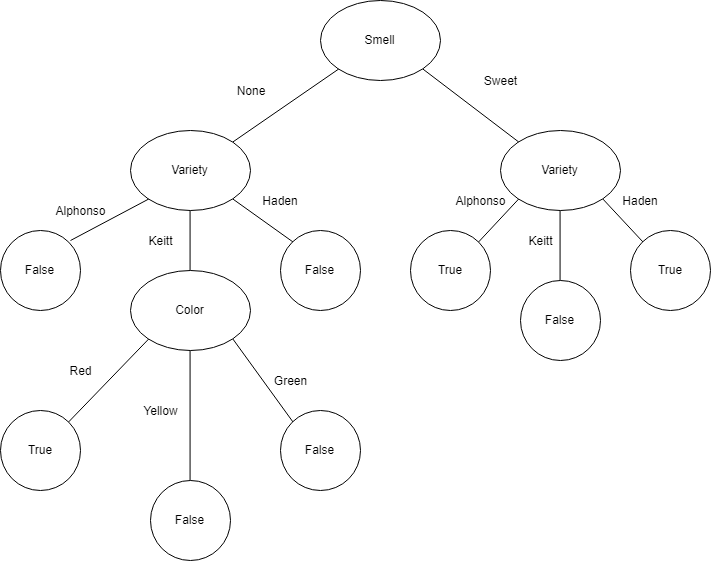
\includegraphics[width=0.7\textwidth]{ml_q2e_uml.png}
  \item~[3 points] Suppose you are given three more examples, listed in Table~\ref{tb-mango-test}. Use your decision tree to predict the label for each example. Also report the accuracy of the classifier that you have learned.
   \begin{table}[h!]
    \centering
    \begin{tabular}{cccc|c|c}
      \hline
      Variety & Color  & Smell  & Time & Ripe? & \textbf{Prediction}\\ \hline
      Alphonso& Green  & Sweet  & Two  & True  & \textbf{True}\\
      Keitt   & Red    & Sweet  & One  & False & \textbf{False}\\
      Haden   & Yellow & None   & Two  & True  & \textbf{False}\\ \hline
    \end{tabular}
    \caption{Test data for mango prediction problem}\label{tb-mango-test}
  \end{table}
   \\\textbf{Ans: }\underline{\textbf{Accuracy} on Test Data Set = 2/3 = \textbf{66.67\%}}
  \end{enumerate}

\item~[10 points] Recall that in the ID3 algorithm, we want to identify the best attribute that splits the examples that are relatively pure in one label.
  Aside from entropy, which we saw in class and you used in the previous question, there are other methods to measure impurity.

  We will now develop a variant of the ID3 algorithm that does not use entropy. If, at some node, we stopped growing the tree and assign the most common label of the remaining examples at that node, then the empirical error on the training set at that node will be
  % 
  $$MajorityError = 1 - \max_{i}p_i$$
  % 
  where, $p_i$ is the fraction of examples that are labeled with the $i^{th}$ label.



  

  \begin{enumerate}
  \item~[2 points]   Notice that $MajorityError$ can be thought of as a measure of impurity just like entropy. Just like we used entropy to define information gain, we can define a new version of information gain that uses $MajorityError$ in place of entropy. Write down an expression that defines a new version of information gain that uses $MajorityError$ in place of entropy.\\\\
    \textbf{Ans: }For Entropy: \\\[Information Gain = H(S) - \sum_{v \in Values(Attributes)}(|S_v|/|S|)* entropy(S_v)\]
    For Majority Error: \\\[New Information Gain = MajorityError(S) - \sum_{v \in Values(Attributes)} (|S_v|/|S|)*MajorityError(S_v) \]
  \item~[6 points] Calculate the value of your newly defined information gain from the previous question for the four features in the mango dataset from ~\ref{tb-mango-train}. Use 3 significant digits. Enter the information gain into Table~\ref{tb-maj-ig}.
    
    \begin{table}[h!]
      \centering
      \begin{tabular}{c|c}
        \hline
        Feature & Information Gain (using majority error) \\ \hline
        Variety & 0.125                 \\
        Color   & 0.125                 \\
        Smell   & 0.25                 \\
        Time    & 0.125                 \\ \hline
      \end{tabular}
      \caption{Information gain for each feature.}\label{tb-maj-ig}
    \end{table}
    ~\\
\textbf{Ans: }MajorityError(S, L=True) = 1 - 4/8 = 1/2\\
\begin{itemize}
\item Variety\\ MajErr(Alphonso) = 1 - 2/4 = 1/2\\ MajErr(Keitt) = 1 - 2/3 = 1/3\\ MajErr(Haden) = 1 - 1 = 0\\
MajErr(Variety) = 1/2 * 1/2 + 3/8 * 1/3 + 0 = 1/4 + 1/8 = 3/8 = 0.375\\
Info Gain = 0.5 - 0.375 = 0.125
\item Color\\ MajErr(Red) = 1 - 2/3 = 1/3 \\ MajErr(Yellow) = 1 - 2/3 = 1/3 \\ MajErr(Green) = 1 - 1/2 = 1/2\\ MajErr(Color) = 3/8 * 1/3 + 3/8 * 1/3 + 1/4 * 1/2 = 1/8 + 1/8 + 1/8 = 3/8 = 0.375\\
Info Gain = 0.5 - 0.375 = 0.125
\item Smell\\ MajErr(None) = 1 - 3/4 = 1/4\\ MajErr(Sweet) = 1 - 3/4 = 1/4\\ MajErr(Smell) = 1/2 * 1/4 + 1/2 * 1/4 = 1/4 = 0.25\\
Info Gain = 0.5 - 0.25 = 0.25
\item Time\\ MajErr(One) = 1 - 2/3 = 1/3\\ MajErr(Two) = 1 - 3/5 = 2/5\\ MajErr(Time) = 3/8 * 1/3 + 5/8 * 2/5 = 1/8 + 1/4 = 3/8 = 0.375\\
Info Gain = 0.5 - 0.375 = 0.125
\end{itemize}
  \item~[2 points] According to your results in the last question, which attribute should be the root for the decision tree?
    Do these two measures (entropy and majority error) lead to the same tree?\\
    \textbf{Ans: }According to Information Gain on majority error, the root node should be ``Time''.\\
   	No the two measures doesn't lead to the same tree, since its differing from the root node itself.
    
  \end{enumerate}

\end{enumerate}


\section{Linear Classifier}
\label{sec:q2}
In the questions in this section, we have four features $x_1, x_2, x_3$ and $x_4$ and the label is represented by $o$.
\begin{enumerate}
    \item~[5 points] Find a linear classifier that correctly classifies the given dataset. You don’t need to run any learning algorithm here. 
Recall that a linear classifier is described by a weight vector $\bw$ and a bias $b$. The classifier predicts 1 if $\bw^T\bx + b \ge 0$ and -1 otherwise.
For this problem, the dataset has 4 features, so the weight vector has 4 components $w_1, w_2, w_3$ and $w_4$. So the linear classifier will
predict 1 if $w_1x_1 + w_2x_2 + w_3x_3 + w_4x_4 + b \ge 0$ and -1 otherwise.
Specify the values of $w_1, w_2, w_3, w_4$ and $b$ that correctly predicts the label for the dataset below.

        \begin{table}[h]
            \centering
            \begin{tabular}{cccc|c}
            $x_1$ & $x_2$ & $x_3$ & $x_4$ & $o$  \\ \hline
            1  & 1  & 1  & 1  &  1  \\
            0  & 1  & 1  & 1  &  1  \\
            1  & 1  & 0  & 0  & -1  \\
            1  & 0  & 0  & 0  & -1  \\
            \end{tabular}
        \end{table}
        \textbf{Ans: }One set of classifiers: \\
$w_1$ = 1, $w_2$ = 1, $w_3$ = 1, $w_4$ = 1 and $b$ = -3\\
$x_1 + x_2 + x_3 + x_4 - 3 \geq 0$ \\
Another set of classifiers:\\
$w_1$ = -1, $w_2$ = -1, $w_3$ = 1, $w_4$ = 1 and $b$ = 0\\
$- x_1 - x_2 + x_3 + x_4 \geq 0$

    \item~[6 points] Suppose the dataset below is an extension of the above dataset.
        Check if your classifier from the previous question correctly classifies the dataset.
        Report its accuracy.

        \begin{table}[h]
        \centering
        \begin{tabular}{cccc|c|c|c}
            x1 & x2 & x3 & x4 & o & Classifier 1 & Classifier 2 \\ \hline
            0  & 0  & 0  & 0  & -1&  -1& 1\\
            0  & 0  & 0  & 1  & -1&  -1& 1\\
            0  & 0  & 1  & 0  & -1&  -1& 1\\
            0  & 0  & 1  & 1  & -1&  -1& 1\\
            1  & 0  & 1  & 1  &  1&   1& 1\\
            1  & 1  & 0  & 1  &  1&   1&-1\\
        \end{tabular}
        \end{table}
\textbf{Ans: }For the given test dataset:\\
Classifier 1: 100\% accuracy\\
Classifier 2: 1/6 = 16.67\% accuracy\\
    \item~[9 points] Given the remaining missing data points of the above dataset in the table below, find a linear classifier that correctly classifies the whole dataset (all three tables together). Specify the values of $w_1, w_2, w_3, w_4$ and $b$ for the classifier.
        \begin{table}[h]
        \centering
        \begin{tabular}{cccc|c}
            x1 & x2 & x3 & x4 & o  \\ \hline
            0  & 1  & 0  & 0  & -1  \\
            0  & 1  & 0  & 1  & -1  \\
            0  & 1  & 1  & 0  & -1  \\
            1  & 0  & 0  & 1  & -1  \\
            1  & 0  & 1  & 0  & -1  \\
            1  & 1  & 1  & 0  &  1  \\
            \end{tabular}
        \end{table}
	\\\textbf{Ans: }Using Classifier 1: we still get 100\% accuracy for the total set of examples. So Classifier 1 with $w_1, w_2, w_3, w_4, b$ = {1, 1, 1, 1, -3} satisfies the entire test/learning data set.
\end{enumerate}


\section{Experiments}
\label{sec:q3}

\subsection*{Cross-Validation}
\begin{enumerate}
    \item~[20 points] \textbf{Implementation}

        For this problem, your will be using the data in \textbf{data} folder.
        This folder contains two files: \textbf{train.csv} and \textbf{test.csv}.
        You will train your algorithm on the training file.
        Remember that you should not look at or use your testing file until your training is complete.
    \begin{enumerate}
        \item~[15 points] Implement the decision tree data structure and the ID3 algorithm for your decision tree (Remember that the decision tree need not be a binary tree!).
        For debugging your implementation, you can use the previous toy examples like the mango data from Table 1.
        Discuss what approaches and design choices you had to make for your implementation and what data structures you used.\\\\
        \textbf{Ans: }I used the concept of classes while creating nodes of the tree and building the decision tree. My tree node has 3 informations: The node type (label or node), based on the attribute type- attribute value (gives the attribute or final label) and dictionary of choices available to that attribute mapped to node objects. \\- Building tree was using the recursive algorithm ID3. The node selection was based on entropy of the attributes on the remaining dataset and information gain for the attributes at each level. \\- Labels were placed based on maximum occurrence of a particular label at that level. \\- Additional usage was on the copy library to do a deep copy of the dictionary in order to be passed down the decision tree. So that any modifications to this data set is not affected in the parent nodes. 
        
        \item~[1 points] Report the error of your decision tree on the \textbf{data/train.csv} file.\\\\
        \textbf{Ans: }The accuracy on the decision tree for the training set was 100\%.
        \item~[1 points] Report the error of your decision tree on the \textbf{data/test.csv} file.\\\\
        \textbf{Ans: }The accuracy on the decision tree for the testing set was 100\%. This is a weird case but it means training set accounted for all possible outcomes which might appear for future cases.
        \item~[3 points] Report the maximum depth of your decision tree.\\\\
        \textbf{Ans: }The maximum depth of the decision tree built was 6. Assuming root node to be counted as depth of 0. Used a recursive algorithm to traverse till the leaf nodes. Return 0 on leaf nodes and at every level return max depth among its children + 1.  
    \end{enumerate}
    
    \item~[20 points] \textbf{Limiting Depth}

        In this section, you will be using 5-fold cross-validation in order to limit the depth of your decision tree, effectively pruning the tree to avoid overfitting.
        You will be using the 5 cross-validation files for this section, titled data/CVfolds/foldX.csv where X is a number between 1 and 5 (inclusive)
        \begin{enumerate}
            \item~[10 points] Run 5-fold cross-validation using the specified files.
            Experiment with depths in the set $\{1,2,3,4,5,10,15\}$, reporting the average cross-validation accuracy and standard deviation for each depth. Explicitly specify which depth should be chosen as the best, and explain why.\\
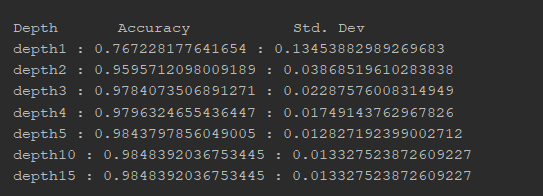
\includegraphics{ml_results.PNG}\\
Looking at the values on Accuracy and standard deviation, it looks like there is not much accuracy improvement from depth 5 to depth 10. And also Standard deviation on depth 5 is the least among all the depths. So picking depth 5 is the best.
            

            \item~[5 points] Using the depth with the greatest cross-validation accuracy from your experiments: train your decision tree on the \textbf{data/train.csv} file. Report the accuracy of your decision tree on the \textbf{data/test.csv} file.\\\\
\textbf{Ans: }Accuracy on train.csv = 99.72\% and accuracy on test.csv = 99.62 \%
            \item~[5 points] Discuss the performance of the depth limited tree as compared to the full decision tree. Do you think limiting depth is a good idea? Why?\\\\
          \textbf{Ans: }Though there is a slight drop in accuracy of 0.2\%, limiting tree is mostly a good idea. This helps minimize over fitting the decision tree to the given training set. There by helps minimize fitting the decision tree to include the noise in the given training data set. Also limiting the tree depth helps speed up learning phase to some extent. 
            
        \end{enumerate}

\end{enumerate}

\section{CS 6350 only: Decision Trees with Attribute Costs}
\label{q4}

\noindent[10 points] Sometimes, we may encounter situations where
the features in our learning problem are associated with costs. For
example, if we are building a classifier in a medical scenario,
features may correspond to the results of different tests that are
performed on a patient. Some tests may be inexpensive (or inflict no
harm), such as measuring the patient's body temperature or
weight. Some other tests may be expensive (or may cause discomfort
to the patient), such as blood tests or radiographs.

In this question, we will explore the problem of learning decision
trees in such a scenario. We prefer decision trees that use features
associated with low costs at the top of the tree and only use higher
cost features if needed at the bottom of the trees.  In order to
impose this preference, we can modify the information gain heuristic
that selects attributes at the root of a tree to penalize costly
attributes.

In this question, we will explore different such variations. Suppose
we denote $Gain(S, A)$ as the information gain of an attribute $A$
for a dataset $S$ (using the original version of information from
ID3). Let $Cost(A)$ denote the cost of the attribute $A$. We can
define two cost-sensitive information gain criteria for attributes
as:

\begin{enumerate}
\item $Gain_T(S, A) = \frac{Gain(S, A)^2}{Cost(A)}$

\item  $Gain_N(S, A) = \frac{2^{Gain(S, A)} - 1}{\sqrt{Cost(A) + 1}}$
\end{enumerate}

In both cases, note that attributes with higher costs are penalized
and so will get chosen only if the information gain is really high.


To evaluate these two methods for root selection, we will use the
following training set:
\begin{center}
  \begin{tabular}{cccc|c}
    \hline
    Shape    & Color  & Size   & Material & Label \\ \hline
    square   & red    & big    & metal    & +     \\
    square   & blue   & small  & plastic  & +     \\
    triangle & yellow & medium & metal    & +     \\
    triangle & pink   & big    & leather  & -     \\
    square   & pink   & medium & leather  & -     \\
    circle   & red    & small  & plastic  & -     \\
    circle   & blue   & small  & metal    & -     \\
    ellipse  & yellow & small  & plastic  & -     \\
    ellipse  & blue   & big    & leather  & +     \\
    ellipse  & pink   & medium & wood     & +     \\
    circle   & blue   & big    & wood     & +     \\
    triangle & blue   & medium & plastic  & +     \\  \hline
  \end{tabular}
\end{center}

Suppose we know the following costs of the attributes:
\begin{center}
  \begin{tabular}{lr}
    Attribute & Cost \\\hline
    Shape     & 10   \\
    Color     & 30   \\
    Size      & 50   \\
    Material  & 100  \\\hline
  \end{tabular}
\end{center}

\begin{enumerate}
\item \relax[8 points] Compute the modified gains $Gain_T$ and $Gain_S$ for each
  attribute using these costs. Fill in your results in the table
  below. (upto 3 decimal places)
  \begin{center}
    \begin{tabular}{l|rr}
      Attribute & $Gain_T$ & $Gain_N$ \\\hline
      Shape     & 0.00037  & 0.013    \\
      Color     & 0.00045  & 0.015    \\
      Size      & 0.00057  & 0.0174   \\
      Material  & 0.00035  & 0.0138   \\\hline
    \end{tabular}
  \end{center}
~\\
Expected Entropy = -7/12 log (7/12) - 5/12 log (5/12) = -0.583*-0.778 - 0.417 * -1.261 - = 0.454 + 0.526 = 0.98

\begin{itemize}
\item Shape\\
Entropy(square) = - 2/3 log (2/3) - 1/3 log (1/3) = -0.667*-0.584 - 0.333 * -1.586 = 0.39 + 0.529 = 0.919\\
Entropy(triangle) = -2/3 log (2/3) - 1/3 log (1/3) = 0.919\\
Entropy(circle) = -1/3 log (1/3) - 2/3 log (2/3) = 0.919\\
Entropy(ellipse) = -1/3 log (1/3) - 2/3 log (2/3) = 0.919\\
Entropy(Shape) = 1/4 * 0.919 * 4 = 0.919\\
Information Gain = 0.98 - 0.919 = 0.061\\
$Gain_T = 0.061^2 / 10 = 0.00037$\\
$Gain_N = (2^{0.061}-1)/\sqrt[]{11} = 0.013$
\item Color\\
Entropy(red) =  - 1/2 log (1/2) - 1/2 log (1/2) = 1\\
Entropy(blue) = - 4/5 log (4/5) - 1/5 log (1/5) = 0.2576 + 0.4644 = 0.722\\
Entropy(yellow) = -1/2 log (1/2) - 1/2 log (1/2) = 1\\
Entropy(pink) = - 2/3 log (2/3) - 1/3 log (1/3) = 0.919\\
Entropy(Color) = 1/6 * 1 + 5/12 * 0.722 + 1/6 * 1 + 1/4 * 0.919 = 0.333 + 0.301 + 0.23 = 0.864\\
Information Gain = 0.98 - 0.864 = 0.116\\
$Gain_T = 0.116^2 / 30 = 0.00045$\\
$Gain_N = (2^{0.116}-1)/\sqrt[]{31} = 0.015$
\item Size\\
Entropy(big) = -3/4 log (3/4) - 1/4 log (1/4) = 0.31125 + 0.5 = 0.81125\\
Entropy(medium) = -3/4 log (3/4) - 1/4 log (1/4) = 0.81125\\
Entropy(small) = -3/4 log (3/4) - 1/4 log (1/4) = 0.81125 \\
Entropy(Size) = 0.81125\\
Information Gain = 0.98 - 0.81125 = 0.169\\
$Gain_T = 0.169^2 / 50 = 0.00057$\\
$Gain_N = (2^{0.169}-1)/\sqrt[]{51} = 0.0174$
\item Material\\
Entropy(metal) = -2/3 log (2/3) - 1/3 log (1/3) = 0.919\\
Entropy(plastic) = -1/2 log (1/2) - 1/2 log (1/2) = 1\\
Entropy(leather) = -2/3 log (2/3) - 1/3 log (1/3) = 0.919\\
Entropy(wood) = 0\\
Entropy(Material) = 1/4 * 0.919 + 1/3*1 + 1/4 * 0.919 = 0.333 + 0.4595 = 0.7925\\
Information Gain = 0.98 - 0.7925 = 0.1875\\
$Gain_T = 0.1875^2 / 100 = 0.00035$\\
$Gain_N = (2^{0.1875}-1)/\sqrt[]{101} = 0.0138$

\end{itemize}
\item \relax[2 points] For each variant of gain, which feature would
  you choose as the root?\\
  \textbf{Ans: }For both variants Size has the maximum Gain. So ``Size'' will be the root node.
\end{enumerate}
\end{document}
